\newcommand{\st}{ \ | \ }

\section{Graph-Based Syntax Definition and Formalisms}
  \label{s:syntax definition}
  In this section we present our graph-based syntax, beginning with the necessary graph theoretic fundamentals to 
  construct the graphs discussed in Sec.~\ref{s:requirements}. 
  The notation used in this paper is adapted from Diestel \cite{Diestel2010}. 
  A \emph{graph} is a pair $G = (V,E)$ of sets such that $E \subseteq V \times V$, 
  which means that the elements of $E$ are 2-element subsets of $V$. The set $V$ 
  contains the \emph{vertices} or \emph{nodes} and the set $E$ contains the \emph{edges}.
  For a \emph{directed graph} (or \emph{digraph}) we construct $E$ as a set of ordered pairs instead 
  of a set of sets. Each ordered pair represents an edge starting at the node 
  indicated by the first entry and directed to the node indicated by the second 
  entry. An edge $e$ = $(x,y)$ may be referred to simply as $xy$. The edges directed out from node $v$ are denoted by $E(v)$ and the edges directed into $v$ are given 
  by $E^{-1}(v)$. 
  If $E$ is not a one-to-one mapping, $E(v)$ may be the empty set, a single node, or a set of nodes.
  \begin{figure}[htb!]
    \begin{center}
    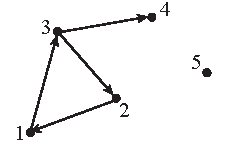
\includegraphics[width=1.5in]{images/example_directed_graph}
    \end{center}
    \vspace{-20pt}
  \caption{Example directed graph.}
  \label{f:example directed graph}
  \end{figure}
  As an example, for the directed graph shown in Fig.~\ref{f:example directed graph} we have
  \begin{IEEEeqnarray*}{rCl}
  V & = & \{1,2,3,4,5\}, \\
  E & = & \big\{(2,1),(3,2),(1,3),(3,4)\big\}.
  \end{IEEEeqnarray*}

  A \emph{path} $P=(V,E)$ from $x_0$ to $x_k$ in graph $G$ is a subgraph of $G$ 
  with $V = \{x_0,x_1,\ldots,x_k\}$ and $E = \{(x_0,x_1),(x_1,x_2),\ldots,(x_{k-1},x_k)\}$. 
Path $P$ is a \emph{cycle} if $x_0 = x_k$.
  A \emph{reverse path} $P_R$ in graph $G$ is a path on $R$, where $R$ is the 
  reverse graph of $G$ obtained by switching the orientation of every edge.


  %does this belong in the analysis block section???? 
  Let $I$ be a nonempty set such that for each $i \in I$ there is a corresponding set $A_i$. 
  The set of sets $\mathcal A = \{A_i \st i \in I\}$ is called an indexed family of sets with index $i$ and 
  indexing set $I$\cite{smith2006}. 
  The union over this family of sets can be described in a few different ways:
  \begin{equation}
  \bigcup_{i \in I} A_i = \bigcup_{A \in \mathcal A} A = \{x \st x \in A \txt{ for some } A \in \mathcal A\}.
  \end{equation}

  Lastly, the cardinality of a set $B$ is the number of elements in $B$ and is denoted as $|B|$.

\subsection{Node and Edge Types}
  \label{ss:types}
Along with these fundamentals of graph theory, we categorize nodes and edges into distinct types in order to provide an intuitive approach to MDAO problem formulation. The three node types are
  \begin{description}
    \item[\bf{variable:}] represents scalar or array data, inputs and outputs,
    \item[\bf{model:}] represents the computation peformed by analysis tools,
    \item[\bf{driver:}] control logic capable of managing iterations (PSG),
  \end{description}
and the three edge types are
%$V_\txt{var}$, $V_\txt{model}$, $V_\txt{driver}$
  \begin{description}
  \item[\bf{connection edge:}] exchange of information external to analysis tools,
  \item[\bf{model edge:}] exchange of information internal to analysis tools,
  \item[\bf{driven edge:}] passing of information from a driver node to a variable node (PSG).
  \end{description}
Figure \ref{f:sellar types} demonstrates the usage of these node and edge types via the Sellar problem. Model nodes are indicated by squares, variable nodes are indicated by circles, connection edges are indicated by dotted lines, and model edges are indicated by solid lines.
\begin{figure}[htb!]
  \begin{center}
    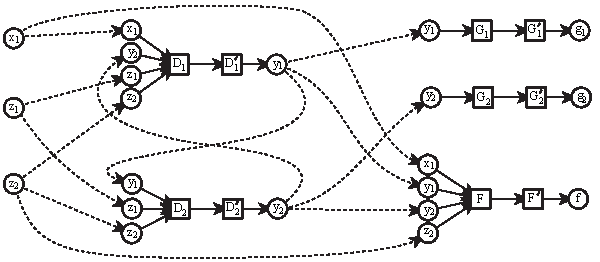
\includegraphics[width=4.0in]{images/sellar_types}
  \end{center}
  \caption{Sellar problem represented as a graph.}
\label{f:sellar types}
\end{figure} 

  A rule set is provided for the usage of these node and edge types to provide a structure to the graph-based representation.
  The driver node and the driven edge are allowed to be present only in PSGs, whereas the other node and edge types can be present in any of the three graph types, 
  subject to the following restrictions: 
  \begin{enumerate}
  \item A model node may have only one edge directed to or from another model node.
  \item A model node may have only model edges directed in or out.
  \item A model node must have at least one edge directed in and at least one edge 
    directed out.
  \item If a variable node has an outgoing model edge, then it may not have other outgoing edges.
  \item If a variable node has an incoming model edge, then it may not have any additional incoming edges.
  \end{enumerate}

  In Alexandrov and Lewis's REMS syntax only two node types (variable and function) 
  and one edge type are included \cite{alexandrov2004}. We have chosen to adopt 
  the terminology ``model'' node instead of ``function'' node to be consistent 
  with modern MDAO framework terminology. The present work adds one additional 
  node type and two additional edge types to the syntax to allow descriptive
  graphs for all three phases of the design problem formulation process indicated in Figs.~\ref{f:tree} and \ref{f:hourglass}.



\subsection{Analysis Blocks}
\label{ss:analysis blocks}
Analysis tools take in a set of input variables and then calculate 
the values for their respective outputs. We represent this process
by a digraph called an \emph{analysis block}; a notional analysis block is shown in Fig.~\ref{f:analysis block}. 
%Each analysis block is a directed graph denoted as $ A=(V_{A},E_{A})$
As indicated in this figure, analysis blocks comprise three sets of nodes representing the distinct local inputs, the analysis (computation), and the distinct local outputs. The local input and local outputs nodes are variable nodes, while the nodes representing the analysis are model nodes. All of the edges within the analysis block are model edges, and are considered fixed to the analysis block. This graph structure demonstrated by Fig.~\ref{f:analysis block} satisfies the rules listed in Sec.~\ref{ss:types}. Reciprocally, the rules ensure that analysis tools are represented via this analysis block structure.
\begin{figure}[htb]
    \begin{center}
    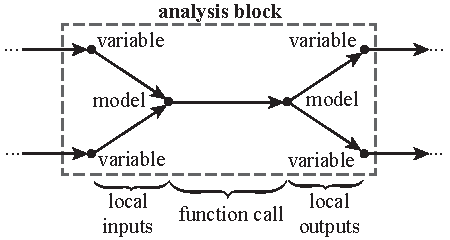
\includegraphics[width=3.0in]{images/analysis_block}
    \end{center}
    \vspace{-10pt}
\caption{Example analysis block with node types labeled.}
\label{f:analysis block}
\end{figure}

The model edge connecting the two model nodes represents the necessary calculations to map the inputs to the outputs of the analysis. 
This edge also provides the opportunity to encode computational cost or other characteristics of the analysis code as a weight in a weighted graph formulation. 
Since all the edges within analysis blocks are fixed, the blocks themselves are fixed sub-graphs within the overall MDAO problem graph. 
The connectivity of nodes and edges in an analysis block cannot be altered for the purposes of MDAO problem formulation; 
however, analysis block sub-graphs can be added or removed from the MDAO problem graph as needed.
Variable nodes in an analysis block can be distinguished as either an input or an output by the manner in which they are connected. 
As shown in Fig.~\ref{f:analysis block}, inputs are represented as variable nodes that have an outgoing edge into a model node, and outputs are represented as variable nodes that have an incoming edge from a model node. 

%MDAO problems require that information be passed between sets of analyses ((DP: needs better transition)).
%For this purpose, connection edges are placed to link analysis blocks
% 
%When information from one output of an analysis block is passed to an 
%input of another analysis block, a new connection edge is added between the two 
%variable nodes involved in the exchange. 
%These connection edges are free, and unlike the edges within an analysis block, the edges can be added or removed depending on the needs of a given design problem. 
%In other words, free connection edges are created by engineers linking an output of one tool to an input of another one. 
%It is allowable for a single output to have outgoing connection edges to multiple downstream inputs. 

\subsection{Objectives, Constraints, and Global Inputs}
\label{ss:objectives and constraints}
Along with analysis tools, objectives, constraints, and global inputs also need to be represented.
In the case of objective functions, a single output value generated by an analysis block could be selected, but commonly multiple values are assembeled together to form a composite objective function. 
Generally, both objective and constraint functions accept a set of inputs and map them to an output value of significance to the overall design problem. 

The operations of implementing composite objective and constraint functions, although typically simple, are effectively identical to the task performed by an analysis block. 
A composite constraint or objective function can therefore be represented as an analysis block within the graph with its own input and output variable nodes. 
Although fundamentally no different than an analysis block, for clarity and convience, it is useful to distinguish between analysis blocks corresponding to analysis codes and those that arise from the addition of objectives or constraints to the graph. 
Therefore, we use an \emph{expression block} to represent an objective or constraint. 
These expression block graphs follow the same structure as analysis blocks presented in Sec.~\ref{ss:analysis blocks}.

Inputs to multiple analysis tools are considered global inputs. These are represented in the graph syntax by single variable nodes refered to as global inputs---the definition of global with respect to a node will be defined subsequently.
%For the sake of consistency of naming conventions $F_j$, $G_j$, and $H_j$ are used to deonte expression blocks for objectives, inequality constraints, and equality constraints. 
%If the relevant objective and constraint values are direct results from other analysis blocks and composite functions are not needed, then expression blocks may be omitted from the MDAO problem graph. 
Figure \ref{f:obj-cons} demonstrates the use of global inputs (black circles), analysis blocks (dotted boxes), and expression blocks (dashed boxes), for the Sellar problem graph.
\begin{figure}[htb!]
  \begin{center}
    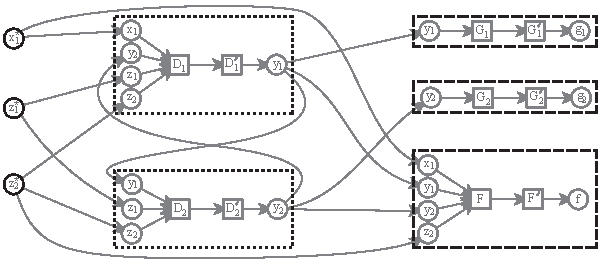
\includegraphics[width=4.0in]{images/sellar_obj_and_cons}
  \end{center}
  \caption{Sellar problem graph indicating global inputs (black circles), analysis blocks (dotted boxes), and expression blocks (dashed boxes).}
\label{f:obj-cons}
\end{figure} 

\subsection{Indegree and Outdegree Limits}
  \label{s:indegree-outdegree}
	To address the MDAO notion of design variables, we first introduce the concept of the degree of a node.
  In a digraph, \emph{indegree} of a node is the number of edges directed in and 
  is denoted as $\txt{deg}^-(v)$, and the \emph{outdegree} 
  is the number of edges directed out and it is denoted as $\txt{deg}^+(v)$ \cite{Diestel2010}.
  In this paper, the indegree and outdegree of a given node refer only to the number of the connection edges 
  directed into or out of the node, respectively. 
%The number of driven edges is not considered relevant because any number 
%  of drivers could be involved in different parts of a solution process. For 
%  example, in a sequential optimization in which a global optimizer is used first 
%  followed by a gradient-based optimizer second to refine global optimizer 
%  result, design variables would have incomming driven edges from both optimizers. 
%  These driven edges would not affect the indegree of those variable nodes. 

  We may now define the \emph{upper indegree limit} 
  \begin{equation}
  \txt{deg}_u^-(v):V \to \mathbb{N}
  \end{equation} 
  and the \emph{lower indegree limit} as
  \begin{equation}
  \txt{deg}_l^-(v):V \to \mathbb{N}.
  \end{equation}
  These user-specified limits govern the number of connection edges that may 
  be directed into a node for a valid graph; of course, $\txt{deg}_l^-(v) \leq \txt{deg}_u^-(v)$ must be satisfied. 
For example, consider a variable 
  node $v$ with $\txt{deg}_u^-(v) = \txt{deg}_l^-(v) = 1$. In this case, $v$ 
  must have exactly one incoming connection edge or the graph is deemed an invalid problem formulation. 

\section{MDAO Constructs Derived from the Graph-Based Syntax}
\label{s:graph representation}
In Sec.~\ref{s:syntax definition} we presented the structure of the graph-based representation. We now discuss how these formalisms provide the remaining MDAO problem constructs identified in Sec.~\ref{s:requirements}.

%To begin, we make use of the Sellar problem, described in 
%Eq. \ref{eqn:simple_fpf} as an example to illustrate the implementation of the syntax. 
%The graph representation of the Sellar problem, using the new stynax, is 
%presented in Fig. \ref{f:sellar_graph_full}. In this section sub-graphs or 
%slight modifications of the full graph will be used to demonstrate the 
%important MDAO constructs described by this graph syntax.
%\begin{figure}[htb!]
%    \begin{center}
%    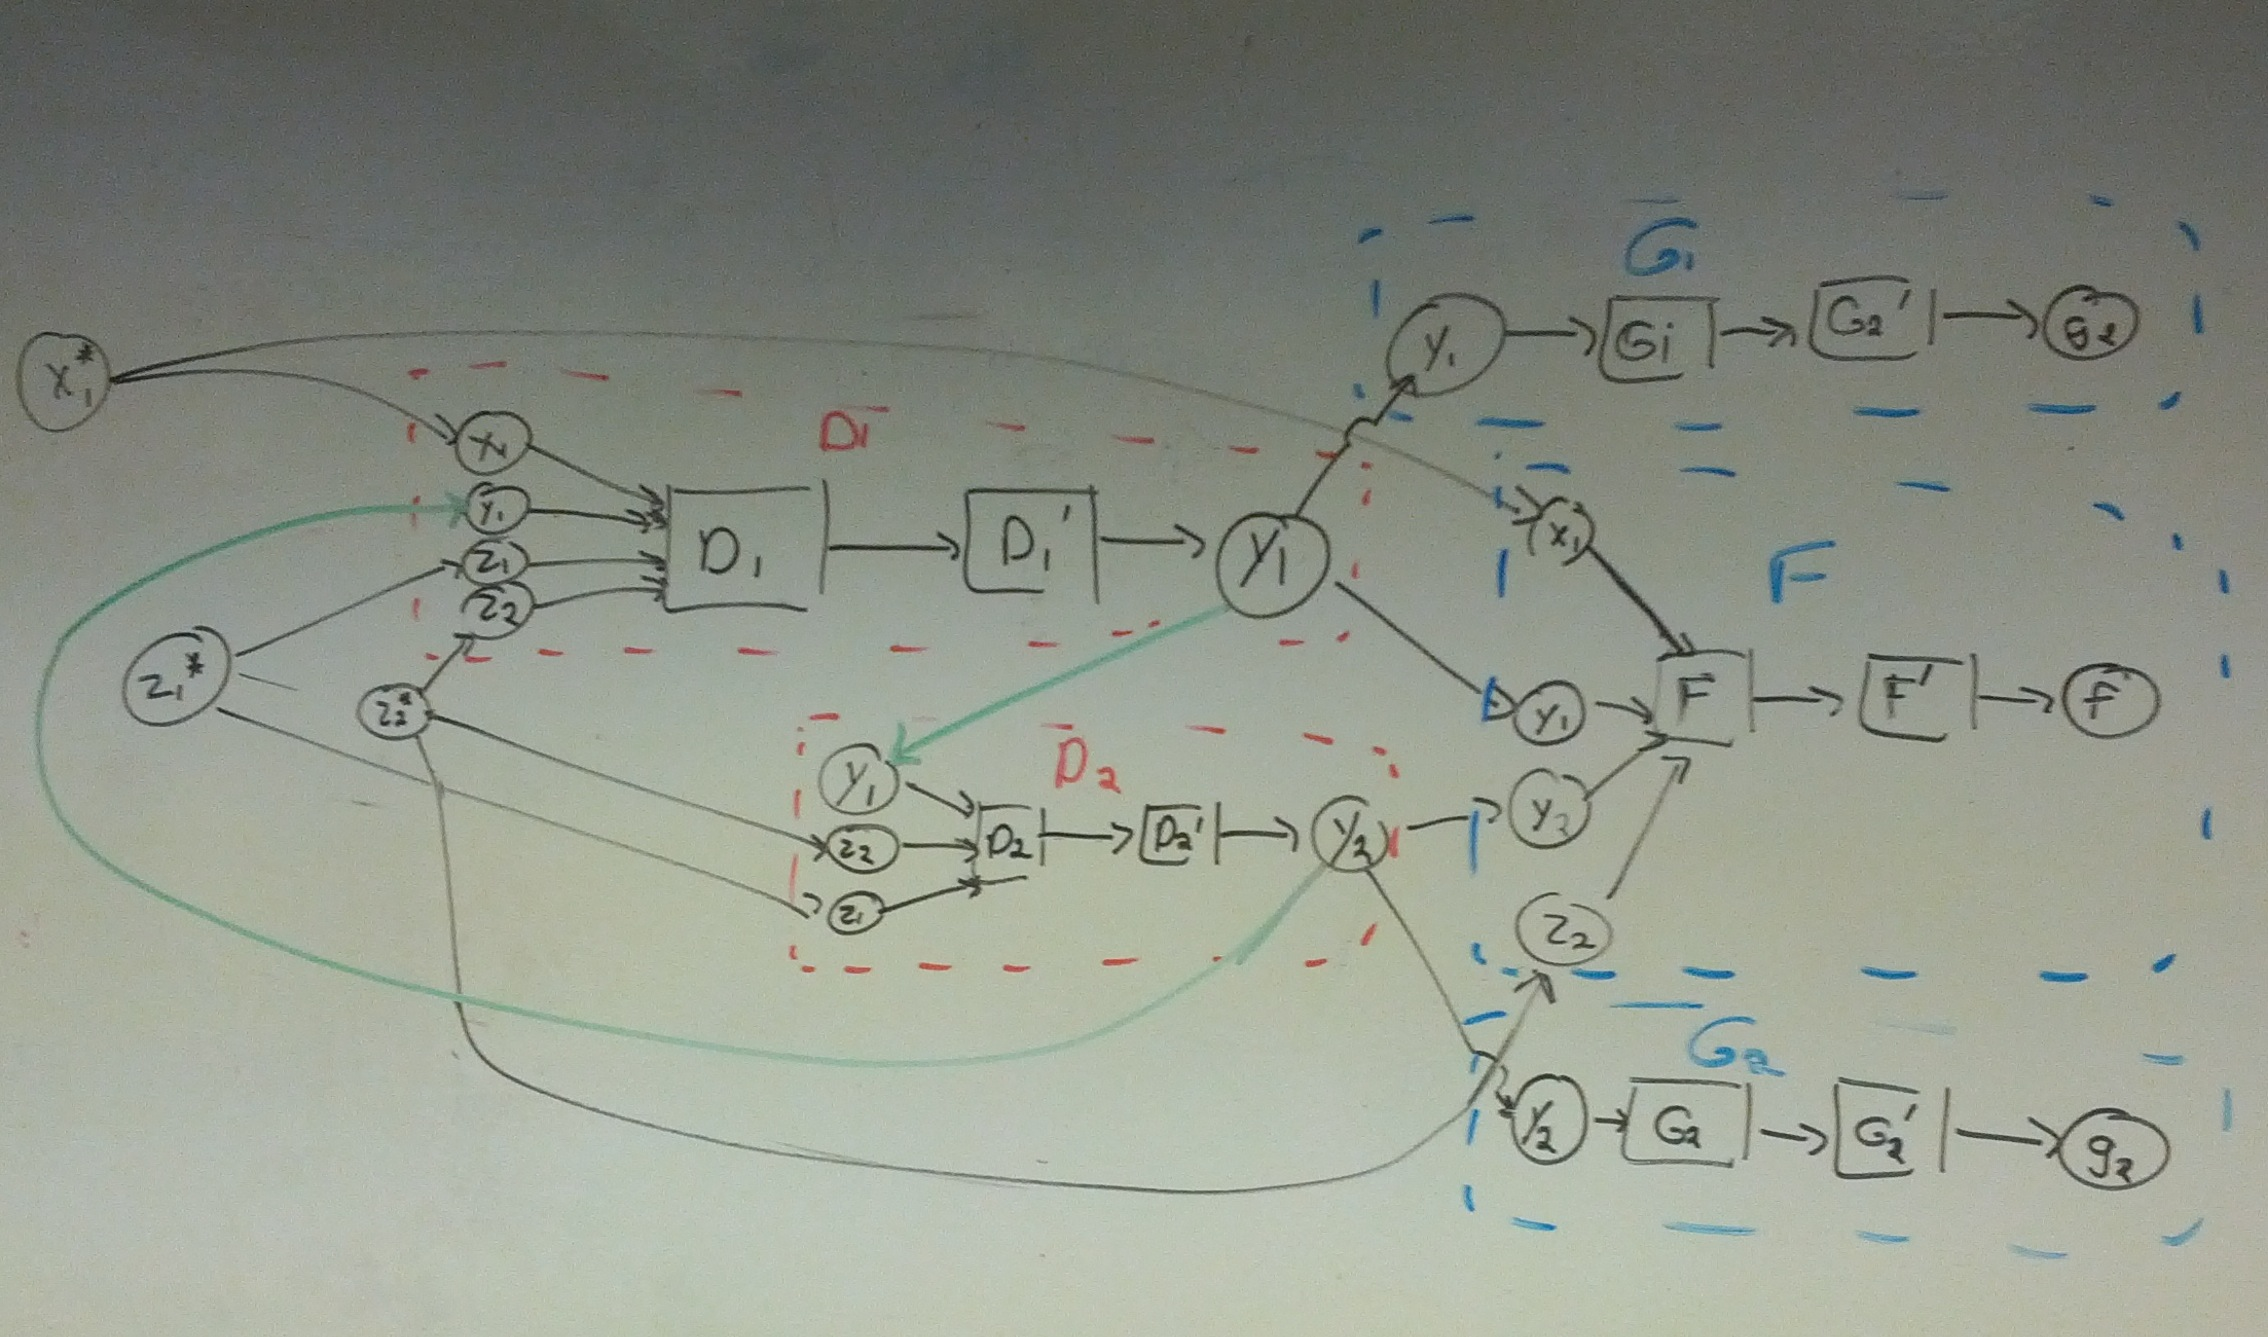
\includegraphics[width=4in]{images/sellar_graph_full}
%    \end{center}
%    \vspace{-10pt}
%\caption{Graph of the Sellar problem formulation}
%\label{f:sellar_graph_full}
%\end{figure}

\subsection{Design Variables, Holes, and Collisions}
Design variables are input variables whose values are free to be 
changed by the designer or by an optimizer in an MDAO study. In the graph-based syntax, a node corresponds to a design variable when the indegree limit of the node is prescribed as zero.

If the indegree limits are violated by the number of incoming connection edges (the indegree of the node), the graph is regarded as an invalid problem formulation. There are two classifications for these violations:
  \begin{description}
    \item[\bf{hole:}] The number of incoming edges is less than the lower indegree limit:
      \begin{equation} 
\txt{deg}^-(v) < \txt{deg}_l^-(v). 
\label{e:hole} 
\end{equation}
      A hole represents a lack of information being supplied to the variable node. This implies that the analysis tool being represented by the analysis block would not be capable of producing outputs.
    \item[\bf{collision:}] The number of incoming edges is greater than the upper indegree limit. 
      \begin{equation} 
\txt{deg}^-(v) > \txt{deg}_u^-(v). 
\label{e:collision}
\end{equation}A collision represents redundant information being supplied to the variable node from two or more sources. This conflict implies an ambiguity as to which information is to be used as an input for the analysis tool.
  \end{description} 

%For the Sellar problem, there are three design variables: $x_1^*$, $z_1^*$, and 
%$z_2^*$. In Fig. \ref{f:designvars} each variable is 
%annotated with the lower indegree limit, and the three design variables are identified 
%in bold((DP:check)). 
%
%\begin{figure}[htb!]
%  \begin{center}
%    [Graph Here....]
%    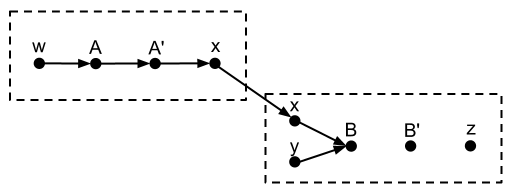
\includegraphics[width=.6\textwidth]{images/design_vars_graph}
%  \end{center}
%  \caption{Sellar problem graph with lower indegree limits for all variables \label{f:designvars}}
%\end{figure}
%
%In Fig. \ref{f:designvars}, the design variable are void of incoming edges. 
%For a valid PSG, design variables could have one or more incoming driven edges representing a value determined by an optimizer. 


  The presence of holes and collisions in a graph represent conflicts that will give
  rise to an invalid problem formulation. It is expected that a maximal connectivity graph will posess these conflicts, whereas a fundamental problem graph will not.

%However, if the graph remains unchanged while the user changes the lower indegree limit of the node to now be zero, then the node becomes a design variable.

%In some cases, the distinction between a hole and a design variable is rather subtle. Both have no incoming connection edges, but 
%
%
%Note that although there are no incoming edges, design variables are not holes 
%in the graph as defined by Eq. \ref{e:hole}. Since they have $\txt{deg}_l^-(v)=0$ 
%having no incoming connection edges does not violate their lower indegree limit. 
%However, the concept of holes can be useful for identifying potential design variables
%given an arbitrary MCG. If you first set $\txt{deg}_l^-(v)=1$ for all variable nodes, 
%and then find the resulint holes, you will have a list of variable nodes that 
%could potentially be design variables. Some variables will be true design variables, 
%while others might represent missing information in the problem formulation. For 
%instance, if there is a hole for a drag input of an aircraft mission analysis code 
%then this is not likely a good choice for a design variable. So it is up to the designer to 
%examine each hole and decide if it's an appropriate design variable. If 
%the variable should become a design variable then set $\txt{deg}_l^-(v)=0$. 
%If a variable should not be a design variable, then leave it as a hole which 
%needs to be addressed in a manner discussed in section \ref{ss:obtaining FPG}.

\subsection{Local vs Global Nodes }

  All global variable nodes have more than one outgoing edge. Conversely all local 
  variable nodes have only a single outgoing edge. Fig.~\ref{f:sellar types} contains 
  three global variables that are not present in the problem formulation given by 
  Eq.~\ref{eqn:simple_fpf}: $x_1^*$, $z_1^*$, and $z_2^*$. The presence of the 
  new nodes is required in order to represent the equality of the given variables that
  was implied by their shared names in Eq.~\ref{eqn:simple_fpf}. 

  The variable $x_1$ is usually refered to as a local variable, which is 
  contradicted by the given graph \cite{Sellar1996}. This discrepancy 
  arises from the explicit treatment of objectives and constraints as separate 
  expression blocks. This variable is could be considered a local 
  variable because it directly affects only analysis block $D_1$. However, by expanding
  $F$ into an expression block with its own inputs, $F$ maintains its own local 
  copy of the $x_1$ variable. This formulation necessitates the creation of the global 
  node $x_1^*$ in the graph with two outgoing edges to link the two $x_1$ inputs nodes 
  in the respective blocks. 

This classification of $x_1^*$ in the Sellar problem
  as a global variable works well within the structure of the Collaborative 
  Optimization (CO) archtiecture \cite{braun1996thesis}. The rules for constructing 
  a problem with CO require that each discipline be given an independent local 
  copy of all global variables. All local variables are retained uniquely 
  within their respective disciplines, except when a local design variable appears 
  explicitely in the objective or global constraint. In this case, a global 
  variable is created and the analysis block is again assigned an 
  independent local copy of it. Following our definition of global and local variable 
  nodes, no such exception for local variables in global expressions is 
  necessary. Whenever a variable is included in an expression block, 
  it forces the creation of a global variable node in the graph which will 
automatically result in the correct CO structure.

  

\subsection{Coupling Between Analyses}
  In MDAO, coupling is the mutual dependence the outputs of two or more analysis 
  codes. In this graph-based syntax, coupling is described by the presence of a 
  cycle between two or more analysis blocks. In the Sellar problem from Eqn \ref{eqn:simple_fpf} 
  a reciprical dependence between $D_1$ and $D_2$ exists through the variabled $y_1$ and $y_2$. 
  The edges belonging to a cycle in the Sellar problem are highlighted in 
  Fig. \ref{f:sellar cycles} where they form a closed path between analysis blocks $D_1$ and $D_2$.

 \begin{figure}[htb!]
  \begin{center}
    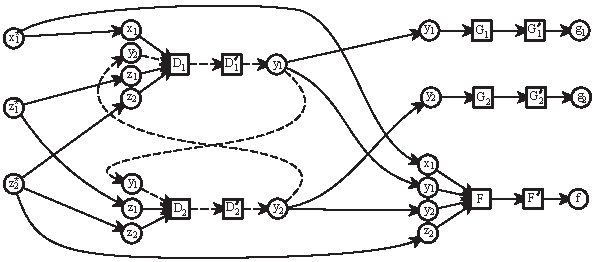
\includegraphics[width=4.0in]{images/sellar_cycles}
  \end{center}
    \caption{Sellar problem graph with dashed edges indicating participation in a cycle.
\label{f:sellar cycles}
    }
\end{figure} 

  Coupling cycles do not contain driver nodes in the MCG or FPG representation. 
  Solvers, optimizers, and other iterative processes are not invovled in the coupling 
  definition; however, one or more solvers will be necessary to build a valid PSG from a given FPG. 
  Additionally, a coupling cycle has no inherent start or end point. It would be acceptable to select
  node in the cycle as a starting point and proceed around the
  loop until the starting point is reached again. For the Sellar Problem, selecting 
  $D_1$ as the starting point would yield a problem as given in 
  Eq.~\ref{eqn:simple}.
  Larger problems can contain more complex cycles in their FPG, indicating more 
  complex coupling between analyses. For example, a cycle can involve more than 
   two analysis blocks. Multiple independent cycles could also exist, indicating 
  independent coupling relationships. Cycles can also overlap, meaning that the same analysis 
  blocks are involved in multiple different coupling cycles. All of these situations
  arise naturally as the size of problems grows, and managing this coupling may
  become difficult. In the present work, Sec.~\ref{s:example problem}
  demonstrates how building an FPG from an MCG provides an opportunity to 
  identify and potentailly reduce the number of cycles in a graph. 

  If many couplings are present, convergence rates can be improved by 
  searching for an effective ordering for the execution of analyses.
  Rogers' DEMAID tool uses a genetic algorithm to find an ordering that minimizes 
  the overall coupling of the system by separating independent cycles in the 
  graph \cite{rogers1996,rogers1996demaid}. Rogers work focused on the matrix 
  form of the DSM for ordering optimization. Lu and Martins more recently leveraged 
  a weighted form of the DSM and used an iterative clustering approach to perform a 
  similar task to DEMAID \cite{Lu2012}.

\subsection{Multi-fidelity Problems}
  \label{ss:multi-fideliy problems}
  A multi-fidelity MDAO problem can be characterized by a formulation in which 
  two or more different analyses each calculating the same data. Multi-fidelity 
  is represented in a graph by a variable node having an indegree greater than 
  one, which means that multiple connection edges are directed into it. When the 
  upper indegree limit of a variable node is set above one, then the node is 
  implied to allow multiple fidelity instances of the variable. When the lower 
  indegree limit of a variable node is set above one, then multiple fidelity instances are required.

  In a multi-fidelity problem, a given variable node may have multiple incoming 
  edges without implying a collision as defined by by Eq.~\ref{e:collision}. 
  Fig.~\ref{f:collision_example} shows a modified version of the Sellar problem 
  with a new analysis, $D_0$, representing a low fidelity version of $D_1$. 
  In this modified graph, the annotations indicate the upper indegree limit. For 
  $D_2$, $\txt{deg}^-_u(D_2.y_1) = 2$ which avoids a collsion. A  
  $\txt{deg}^-_u(v) > 1$ for any variable in a graph represents a decision to 
  allow multiple fidelities to interact at that part of the graph in order to allieviate
  a conflict. In section \ref{ss:obtaining FPG} we present an algorithm for finding 
  conflicts within a given MCG so that a designer can make the necessary decisisons about each 
  one in turn. 
  \begin{figure}
    \begin{center}
      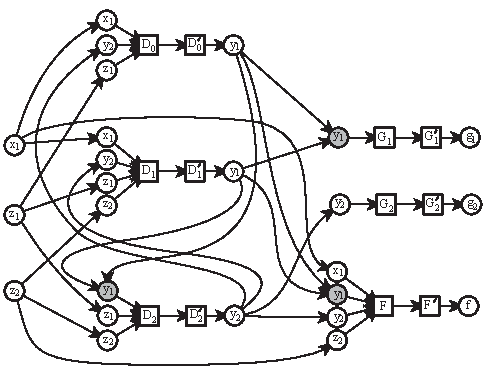
\includegraphics[width=4in]{images/sellar_mulfi}
    \caption{Graph of the modified Sellar, multi-fidelity problem with $\txt{deg}^-_u(v)$ annotations on variable nodes\label{f:collision_example}}
  \end{center}
  \end{figure}

  Multi-fidelity problems are always charaterized by graphs with variable 
  nodes that have an $\txt{deg}^-_u(v) > 1$. These problems require 
  special techniques for resolving the confliciting edges by introducing some mechanism
  to manage when each of the different fidelity analyses are 
  run\cite{march2012provably,alexandrov2001approximation,Huang_Allen_Notz_Miller_2006}.
  The specifics of this mechanism are not given in any form withing an MCG or 
  FPG. Instead the multi-fidelity mechanism specifics would be represented as a 
  driver in a PSG derived from a multi-fidelity FPG. 

Table \ref{t:variable node classification} provides examples to summarize the classification of a variable node as a hole, design variable, single valid input (nominal), collision, or multi-fidelity.

\begin{table}[htbp]
  \centering
  \caption{Variable Node Classification}
    \begin{tabular}{ccccc}
    \toprule
    $\txt{deg}^-_l(v)$ & $\txt{deg}^-_u(v)$ & $\txt{deg}^-(v)$ & valid & classification \\
    \midrule
    0     & 0     & 0     & yes   & design variable \\
    0     & 0     & 1     & yes   & collision \\
    0     & 1     & 0     & yes   & design variable \\
    0     & 1     & 1     & yes   & single input \\
    1     & 1     & 0     & no    & hole \\
    1     & 1     & 1     & yes   & single input \\
    1     & 1     & $>1$ & no    & collision \\
    1     & 2     & 1     & yes   & supplied input \\
    1     & 2     & 2     & yes   & multi-fidelity \\
    2     & 2     & $<2$ & no    & hole \\
    2     & 2     & 2     & yes   & multi-fidelity \\
    2     & 2     & $>2$     & no   & collision \\
    \bottomrule
    \end{tabular}%
  \label{t:variable node classification}%
\end{table}%



